\documentclass[tikz,border=20pt]{standalone}
\usetikzlibrary{calc,arrows.meta,positioning,shapes.geometric}
\usepackage{amsmath,amssymb}

\begin{document}
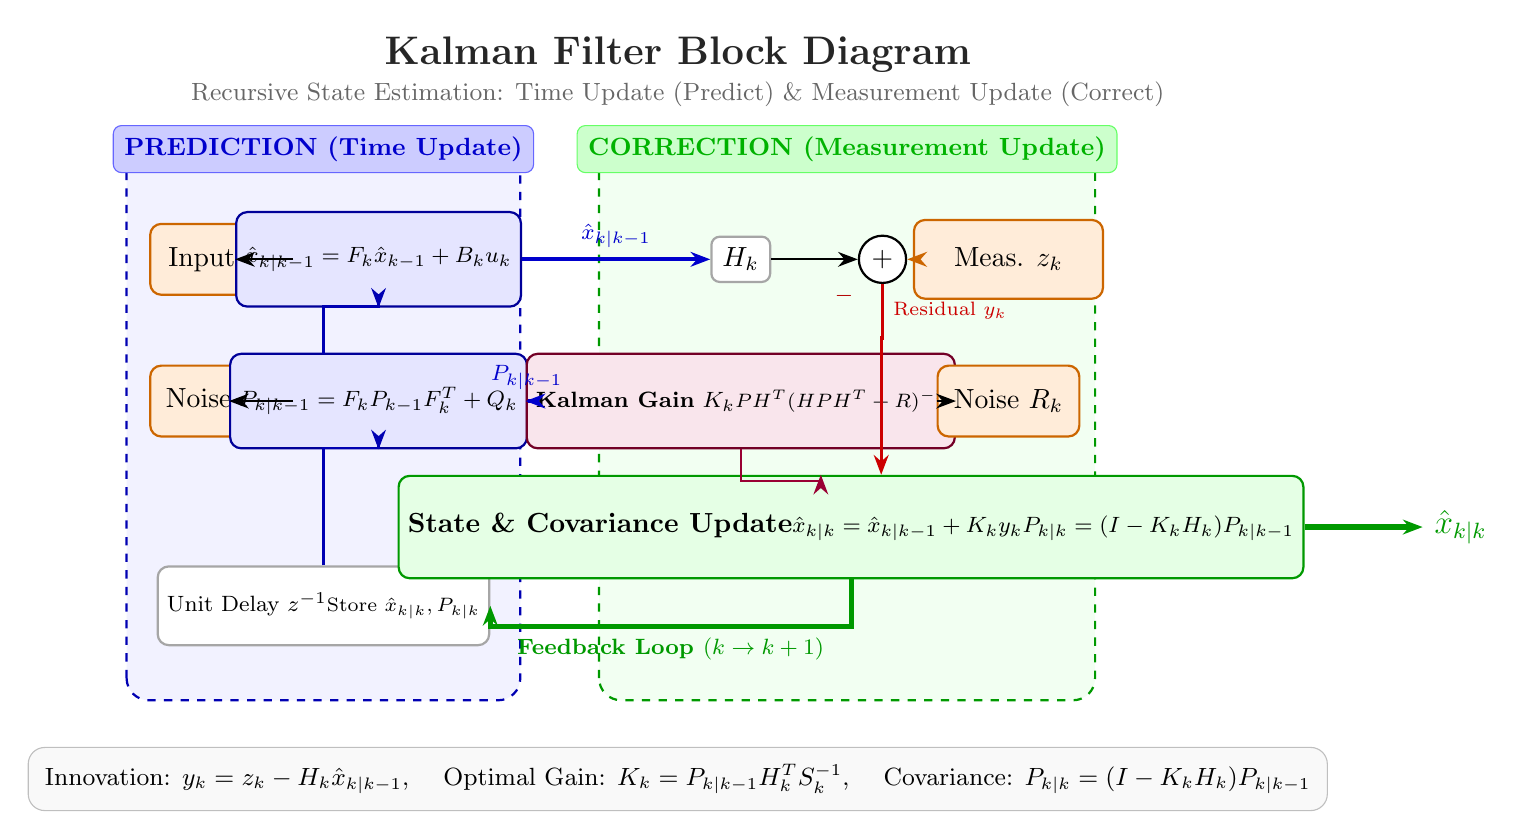
\begin{tikzpicture}[
  x=1cm, y=1cm, >=Stealth,
  block/.style={rectangle, draw=blue!60!black, fill=blue!10, thick, rounded corners=4pt, text centered, minimum width=3.2cm, minimum height=1.2cm},
  greenblock/.style={rectangle, draw=green!60!black, fill=green!10, thick, rounded corners=4pt, text centered, minimum width=3.2cm, minimum height=1.2cm},
  purpleblock/.style={rectangle, draw=purple!60!black, fill=purple!10, thick, rounded corners=4pt, text centered, minimum width=3.2cm, minimum height=1.2cm},
  amberblock/.style={rectangle, draw=orange!80!black, fill=orange!15, thick, rounded corners=4pt, text centered, minimum width=2.4cm, minimum height=1.0cm},
  sum/.style={circle, draw=black, thick, fill=white, inner sep=0pt, minimum size=6mm},
  line/.style={draw, thick, -{Stealth[length=2.5mm]}}
]

  % Title
  \node[font=\bfseries\Large, text=black!85] at (5.2, 5.0) {Kalman Filter Block Diagram};
  \node[font=\small, text=gray!80!black] at (5.2, 4.5) {Recursive State Estimation: Time Update (Predict) \& Measurement Update (Correct)};

  % SECTION 1: PREDICTION (TIME UPDATE) - Left Stage
  \draw[blue!70!black, thick, dashed, fill=blue!5, rounded corners=8pt] (-1.8, -3.2) rectangle (3.2, 3.8);
  \node[font=\bfseries\small, text=blue!80!black, fill=blue!20, draw=blue!60, rounded corners=3pt, inner sep=4pt] at (0.7, 3.8) {PREDICTION (Time Update)};

  % Control input u_k
  \node[amberblock, minimum width=1.8cm, minimum height=0.9cm] (uk) at (-0.6, 2.4) {Input $u_k$};
  % State prediction block
  \node[block] (xpred) at (1.4, 2.4) {\footnotesize $\hat{x}_{k|k-1} = F_k \hat{x}_{k-1} + B_k u_k$};

  % Process noise Q_k
  \node[amberblock, minimum width=1.8cm, minimum height=0.9cm] (qk) at (-0.6, 0.6) {Noise $Q_k$};
  % Covariance prediction block
  \node[block] (ppred) at (1.4, 0.6) {\footnotesize $P_{k|k-1} = F_k P_{k-1} F_k^T + Q_k$};

  % Unit delay feedback
  \node[rectangle, draw=gray!70, fill=white, thick, rounded corners=4pt, text centered, minimum width=2.8cm, minimum height=1cm] (delay) at (0.7, -2.0) {
    \footnotesize Unit Delay $z^{-1}$ \\ \scriptsize Store $\hat{x}_{k|k}, P_{k|k}$
  };

  % Connectors within prediction
  \draw[line] (uk) -- (xpred);
  \draw[line] (qk) -- (ppred);
  \draw[line, blue!70!black] (delay.north) -- (0.7, 0.0) -| (ppred.south);
  \draw[line, blue!70!black] (0.7, 1.2) -- (0.7, 1.8) -| (xpred.south);

  % SECTION 2: UPDATE (MEASUREMENT UPDATE) - Right Stage
  \draw[green!60!black, thick, dashed, fill=green!5, rounded corners=8pt] (4.2, -3.2) rectangle (10.5, 3.8);
  \node[font=\bfseries\small, text=green!70!black, fill=green!20, draw=green!60, rounded corners=3pt, inner sep=4pt] at (7.35, 3.8) {CORRECTION (Measurement Update)};

  % Measurement z_k
  \node[amberblock] (zk) at (9.4, 2.4) {Meas. $z_k$};
  % Summing node for residual
  \node[sum] (sumres) at (7.8, 2.4) {$+$};
  \node[below left=1pt of sumres, font=\footnotesize\bfseries, text=red!70!black] {$-$};

  % Measurement matrix H_k
  \node[rectangle, draw=gray!70, fill=white, thick, rounded corners=3pt, inner sep=4pt] (hk) at (6.0, 2.4) {$H_k$};

  % Kalman Gain block K_k
  \node[purpleblock, minimum width=3.4cm] (gain) at (6.0, 0.6) {
    \footnotesize \textbf{Kalman Gain} $K_k$ \\ \scriptsize $P H^T (H P H^T + R)^{-1}$
  };

  % Measurement noise R_k
  \node[amberblock, minimum width=1.8cm, minimum height=0.9cm] (rk) at (9.4, 0.6) {Noise $R_k$};

  % State & Covariance Update
  \node[greenblock, minimum width=4.8cm, minimum height=1.3cm] (update) at (7.4, -1.0) {
    \textbf{State \& Covariance Update} \\
    \footnotesize $\hat{x}_{k|k} = \hat{x}_{k|k-1} + K_k y_k$ \\
    \footnotesize $P_{k|k} = (I - K_k H_k) P_{k|k-1}$
  };

  % INTER-STAGE CONNECTIONS
  % x_hat_{k|k-1} forward
  \draw[line, blue!80!black, line width=1.5pt] (xpred.east) -- (hk.west) node[midway, above, font=\footnotesize] {$\hat{x}_{k|k-1}$};
  \draw[line] (hk.east) -- (sumres.west);
  \draw[line, orange!80!black, line width=1.2pt] (zk.west) -- (sumres.east);

  % Residual arrow down to update
  \draw[line, red!80!black, line width=1.2pt] (sumres.south) -- (7.8, 1.4) node[midway, right, font=\scriptsize, text=red!80!black] {Residual $y_k$} -| (update.60);

  % P_{k|k-1} forward
  \draw[line, blue!80!black, line width=1.5pt] (ppred.east) -- (gain.west) node[midway, above, font=\footnotesize] {$P_{k|k-1}$};
  \draw[line] (rk.west) -- (gain.east);
  \draw[line, purple!80!black] (gain.south) -- ++(0, -0.4) -| (update.120);

  % FEEDBACK LOOP
  \draw[line, green!60!black, line width=1.8pt] (update.south) -- ++(0, -0.6) -| (delay.east)
    node[pos=0.25, below, font=\footnotesize\bfseries, text=green!60!black] {Feedback Loop $(k \rightarrow k+1)$};

  % OUTPUT ESTIMATE ARROW
  \draw[line, green!60!black, line width=2pt] (update.east) -- ++(1.5, 0)
    node[right, font=\large\bfseries, text=green!60!black] {$\hat{x}_{k|k}$};

  % Formula Summary Note at bottom
  \node[draw=gray!50, fill=gray!5, rounded corners=6pt, font=\small, inner sep=6pt] at (5.2, -4.2) {
    Innovation: $y_k = z_k - H_k \hat{x}_{k|k-1}, \quad$ Optimal Gain: $K_k = P_{k|k-1} H_k^T S_k^{-1}, \quad$ Covariance: $P_{k|k} = (I - K_k H_k) P_{k|k-1}$
  };

\end{tikzpicture}
\end{document}
